\include{head}
\begin{document}


\begin{center}
    \Large{Задание 1}\\
    Стрижак Даниил
\end{center}
\section{Распределение Максвелла}
Из-за того, что в системе рассматривается всего 1000 частиц, то распределение Максвелла не установится никогда, но имеет смысл говорить о том, когда распределение будет "очень похоже" на Максвелловское. \\

Посмотрим на линеаризованную зависимость расперделения по модулям скоростей, т.е. зависимость $\ln{\frac{N}{V^2}}$ от $V^2$, где N -- количество частициц в промежутке, равном 0.1 от разницы между наибольшим и наименьшим значениям  (Метод простой скользящей средней).  \\

Ниже приведены зависимости при K = 2, 10, 50 и 80 шагов интегрирования:

\begin{minipage}{0.47\textwidth}
    \begin{center}
        \includegraphics[width=\linewidth]{1.png}\\
        2 шага
    \end{center}
   
\end{minipage}
\begin{minipage}{0.47\textwidth}
    \begin{center}
        \includegraphics[width=\linewidth]{10.png}\\
        10 шагов
    \end{center}
\end{minipage}

\begin{minipage}{0.47\textwidth}
    \begin{center}
        \includegraphics[width=\linewidth]{30.png}\\
        30 шагов
    \end{center}
\end{minipage}
\begin{minipage}{0.47\textwidth}
    \begin{center}
        \includegraphics[width=\linewidth]{80.png}\\
        80 шагов
    \end{center}
\end{minipage}

\newpage

После 80 шага можно считать, что распределение Максвелла почти установилось. Нелинеарезированное распределение выглядит так:

\begin{center}
        \includegraphics[width=0.6\linewidth]{Maxwell.png}\\
\end{center}

А распределения по модулям скоростей так:\\


\begin{minipage}{0.47\textwidth}
    \begin{center}
        \includegraphics[width=\linewidth]{Maxwell_pr.png}\\
        30 шагов
    \end{center}
\end{minipage}
\begin{minipage}{0.47\textwidth}
    \begin{center}
        \includegraphics[width=\linewidth]{Maxwell_pr_lin.png}\\
        80 шагов
    \end{center}
\end{minipage}

\ 

\newline

На самом деле распределение Максвелла -- один из критериев установившегося равновесия в системе и говорить о том, что оно установилось стоит только тогда, когда все критерии будут удовлетворять теории. Один из них обсуждается в следующем пункте; после установления равновесия будет установлено и распределение Максвелла в максимально близком приближении к реальности. При времени перерасчета dt = 0,0001 количество шагов примерно равно 4000. 

\newpage

\section{Время динамической памяти}

Для расчета времени динамической памяти стоит запустить симуляцию при двух разных временах перерасчета  $dt_1 = 0.0001$ и $dt_2 = 0.001$ и посчитать невязки скоростей и радиус-векторов: $<(v_1 - v_2)^2>(t)$ и $<(r_1 - r_2)^2>(t)$. Кривые выходят на плато на 4000 шаге т. е. 0,4 секунды собственного времени. 

\begin{center}
        \includegraphics[width=\linewidth]{Residuals.png}\\
\end{center}

\section{Уравнения состояния}
\subsection{Зависимости разных величин от плотности}

При температуре Т = 2.0 запустим программу несколько раз, рассчитав давление, как среднее значение величины $P = P_m + P_f$, начиная с 4000 шага до последнего. 

$$<P_f> =\frac{1}{3V}< \sum\limits_{j = 0}^N\sum\limits_{i<j}\mathbf{F_{ij}}\cdot \mathbf{r_{ij}} > $$
$$<P_m> = \frac{3N}{2V}<E_k> $$

\newpage

Полученные данные, путем моделирования вынесены в таблицу:\\

\begin{center}
\begin{tabular}{|c|c|c|c|c|}
\hline
\ & \ & \ & \ & \ \\
$\frac{L}{2}$ &Давление & Сжимаемость &$ \frac{P_{кинет.}}{P_{кинет.} + P_{потенц.}} $& Плотность\\
 \ & \ & \ & \ \\
\hline
5.30 &43.87 & -- & 0.154 & 0.839 \\
\hline
5.35 &37.28 & 0.479&0.166  & 0.816 \\
\hline
5.40 &32.18 &0.679 &0.176  & 0.793 \\
\hline
5.45 &29.10 & 0.849&0.187  & 0.772\\
\hline
5.50 &25.70 &0.798 &0.196  & 0.751 \\
\hline
5.55 &22.27 &1.051 &0.210  & 0.731\\
\hline
5.60 &20.56 &1.157 &0.216  & 0.711\\
\hline
5.65 &17.64 &1.258 &0.230  & 0.693\\
\hline
5.70 &16.34 &2.096 &0.238  & 0.674\\
\hline
5.75 &15.13 &1.983 &0.247  & 0.657\\
\hline
5.80 &13.71 &2.486 &0.259  & 0.640\\
\hline
5.85 &13.05 &2.842 &0.263  & 0.624\\
\hline
5.90 &12.26 &3.008 &0.272  & 0.608\\
\hline
5.95 &11.36 &2.533 &0.280  & 0.593\\
\hline
6.00 &10.27 &2.590  & 0.292 & 0.578\\
\hline
6.05 &9.43 &3.443 &0.301  &0.564 \\
\hline
6.10 &8.83 &3.786  &0.309 & 0.550\\
\hline
6.15 &8.58 &4.134 &0.313  &0.537 \\
\hline
6.20 &7.88  &4.171  & 0.320 & 0.524\\
\hline
6.25 &7.42 &4.138 &0.332  &0.512 \\
\hline
6.30 &6.72 &4.070 &0.343  &0.500 \\
\hline
6.35 &6.25 &4.820 &0.348  &0.488 \\
\hline
6.40 &5.74 &4.510 &0.360  &0.477 \\
\hline
6.45 &5.53 &5.074 &0.364  &0.466 \\
\hline
6.50 &5.53 &5.241 &0.363  &0.455 \\
\hline
6.55 &5.25 &5.896 &0.373 &0.445 \\
\hline
6.60 &4.67 &5.611 &0.386  &0.434 \\
\hline
6.65 &4.44 &6.044 &0.392  &0.425 \\
\hline
6.70 &4.28 &6.206 &0.392& 0.415\\
\hline
6.75 &3.95 &6.084 &0.409 &0.406 \\
\hline
6.80 &3.60 &6.001 &0.420 &0.398 \\
\hline
6.85 &3.54 &6.056 &0.419  &0.389 \\
\hline
6.90 &3.57 &6.038 &0.416  &0.381 \\
\hline
6.95 &3.39 &5.995 &0.428  &0.372 \\
\hline
7.00 &3.23 & -- &0.431  & 0.364\\
\hline
\end{tabular}
\end{center}


\newpage

Для расчета сжимаемости $\beta = -\frac{1}{V}\left(\frac{\partial V}{\partial P} \right)_T$ воспользуемся методом сплайнов 3 степени, чтобы рассчитать производную $\left(\frac{\partial V}{\partial P} \right)_T$. \\



Построим полученные зависимости давления от плотности $P(\rho)$ (слева) и сжимаемости от плотности $\beta(\rho)$ (справа):\\

\newline

\begin{minipage}{0.47\textwidth}
\begin{center}
		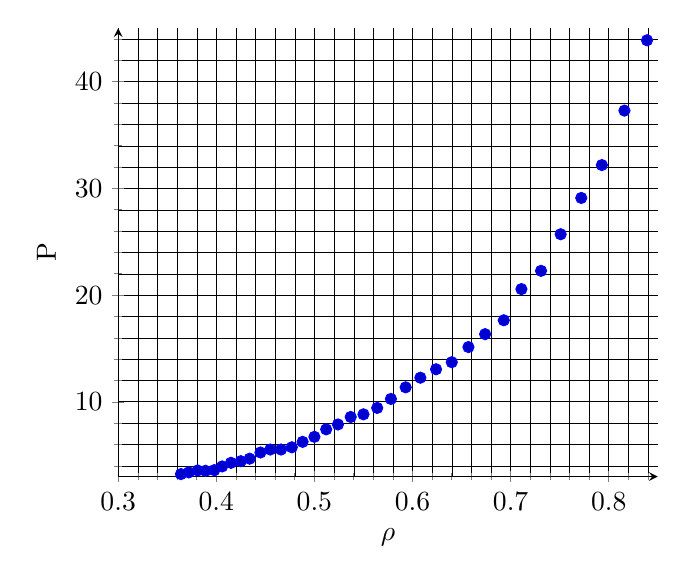
\begin{tikzpicture}[scale = 1.0]
		\begin{axis}[
		axis lines = left,
		ylabel = {P},
		xlabel = {$\rho$},
		minor grid style={black, line width=0.05pt},
		major grid style={solid,black, line width=0.3pt},
		xmin=0.3, xmax=0.85,
		ymin=3, ymax=45,
		ymajorgrids = true,
		xmajorgrids = true,
		yminorgrids = true,
		xminorgrids = true,
		minor tick num = 4
		]
		\addplot+[only marks ] plot[error bars/.cd, y dir=both, y explicit]
		coordinates {
			(0.839,43.87)
			(0.816, 37.28)
			(0.793, 32.18)
			(0.772, 29.10)
			(0.751, 25.70)
			(0.731, 22.27)
			(0.711, 20.56)
			(0.693, 17.64)
			(0.674, 16.34)
			(0.657, 15.13)
			(0.640, 13.71)
			(0.624, 13.05)
			(0.608, 12.26)
			(0.593, 11.36)
			(0.578, 10.27)
			(0.564, 9.43)
			(0.550, 8.83)
			(0.537, 8.58)
			(0.524, 7.88)
			(0.512, 7.42)
			(0.500, 6.72)
			(0.488, 6.25)
			(0.477, 5.74)
			(0.466, 5.53)
			(0.455, 5.53)
			(0.445, 5.253)
			(0.434, 4.673)
			(0.425, 4.438)
			(0.415, 4.284)
			(0.406, 3.95)
			(0.398, 3.6)
			(0.389, 3.54)
			(0.381, 3.57)
			(0.372, 3.39)
			(0.364, 3.23)
		};
		

		\end{axis}

		\end{tikzpicture}
		
\end{center}

\end{minipage}
\begin{minipage}{0.47\textwidth}
\begin{center}
		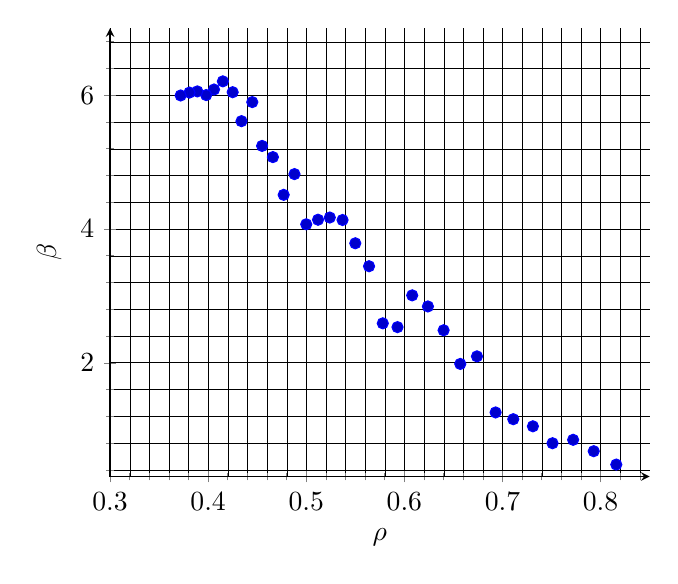
\begin{tikzpicture}[scale = 1.0]
		\begin{axis}[
		axis lines = left,
		ylabel = {$\beta$},
		xlabel = {$\rho$},
		minor grid style={black, line width=0.05pt},
		major grid style={solid,black, line width=0.3pt},
		xmin=0.3, xmax=0.85,
		ymin=0.3, ymax=7,
		ymajorgrids = true,
		xmajorgrids = true,
		yminorgrids = true,
		xminorgrids = true,
		minor tick num = 4
		]
		\addplot+[only marks ] plot[error bars/.cd, y dir=both, y explicit]
		coordinates {
			
			(0.816, 0.479)
			(0.793, 0.679)
			(0.772, 0.849)
			(0.751, 0.798)
			(0.731, 1.051)
			(0.711, 1.157)
			(0.693, 1.258)
			(0.674, 2.096)
			(0.657, 1.983)
			(0.640, 2.486)
			(0.624, 2.842)
			(0.608, 3.008)
			(0.593, 2.533)
			(0.578, 2.590)
			(0.564, 3.443)
			(0.550, 3.786)
			(0.537, 4.134)
			(0.524, 4.171)
			(0.512, 4.138)
			(0.500, 4.070)
			(0.488, 4.820)
			(0.477, 4.51)
			(0.466, 5.074)
			(0.455, 5.241)
			(0.445, 5.896)
			(0.434, 5.611)
			(0.425, 6.044)
			(0.415, 6.206)
			(0.406, 6.084)
			(0.398, 6.001)
			(0.389, 6.056)
			(0.381, 6.038)
			(0.372, 5.995)
			
		};
		

		%\addplot[blue, domain=0:30]{2*x};
		\end{axis}

		\end{tikzpicture}
		
\end{center}

\end{minipage}

\

\newline

Можно заметить, что при малой плотности зависимость давления от плотности является линейной, что так же подтверждается независимостью значения сжимаемости от плотности в диапазоне до 0.42 условных единиц плотности. \\

Так же построим зависимость $\frac{P_{кинет.}}{P_{кинет.} + P_{потенц.}}(\rho) $:\\

\begin{center}
\begin{tikzpicture}[scale = 1.3]
		\begin{axis}[
		axis lines = left,
		ylabel = {$\frac{P_{кинет.}}{P_{кинет.} + P_{потенц.}} $},
		xlabel = {$\rho$},
		minor grid style={black, line width=0.05pt},
		major grid style={solid,black, line width=0.3pt},
		xmin=0.3, xmax=0.85,
		ymin=0.15, ymax=0.45,
		ymajorgrids = true,
		xmajorgrids = true,
		yminorgrids = true,
		xminorgrids = true,
		minor tick num = 4
		]
		\addplot+[only marks ] plot[error bars/.cd, y dir=both, y explicit]
		coordinates {
			(0.839,0.154)
			(0.816, 0.166)
			(0.793, 0.176)
			(0.772, 0.187)
			(0.751, 0.196)
			(0.731, 0.210)
			(0.711, 0.216)
			(0.693, 0.230)
			(0.674, 0.238)
			(0.657, 0.247)
			(0.640, 0.259)
			(0.624, 0.263)
			(0.608, 0.272)
			(0.593, 0.280)
			(0.578, 0.292)
			(0.564, 0.301)
			(0.550, 0.309)
			(0.537, 0.313)
			(0.524, 0.320)
			(0.512, 0.332)
			(0.5, 0.343)
			(0.488, 0.348)
			(0.477, 0.360)
			(0.466, 0.364)
			(0.455, 0.363)
			(0.445, 0.373)
			(0.434, 0.386)
			(0.425, 0.392)
			(0.415, 0.392)
			(0.406, 0.409)
			(0.398, 0.42)
			(0.389, 0.419)
			(0.381, 0.416)
			(0.372, 0.428)
			(0.364, 0.431)
		};
		

		%\addplot[blue, domain=0:30]{2*x};
		\end{axis}

		\end{tikzpicture}
		\end{center}

\newpage
\subsection{Обрезка потенциала}

При обрезке потенциала стоит ввести добавочное давление:

$$ \Delta \mathrm{P}^{\text {tail }} =(1 / 2) 4 \pi \rho^{2} \int_{r_{c}}^{\infty} \operatorname{dr} r^{2} \mathbf{r} \cdot \mathbf{f}(r)  =\frac{16}{3} \pi \rho^{2} \epsilon \sigma^{3}\left[\frac{2}{3}\left(\frac{\sigma}{r_{c}}\right)^{9}-\left(\frac{\sigma}{r_{c}}\right)^{3}\right] $$

Для проверки данной формулы достаточно провести измерения для 7 различных $r_{cut}$ при объеме 1728 условных единиц (длина стороны куба равна 12, $P_0 = 10.27$):


\begin{center}
\begin{tabular}{|c|c|c|c|c|}
\hline
\ & \ & \ & \ & \ \\
r_{cut} &P & $\Delta P$ &$P^{теор}$& ошибка\\
 \ & \ & \ &  &\ \\
\hline
5.5&10.33 & -0.06&-0.058 &3.4\% \\
\hline
5.0&10.35 & -0.08&-0.078 &2.5\% \\
\hline
4.5&10.37 & -0.10&-0.106 &5.6\% \\
\hline
4.0&10.44 &-0.16 &-0.151 &5.9\% \\
\hline
3.5&10.48 &-0.21 &-0.226 &7.0\% \\
\hline
3.0&10.65 &-0.38 &-0.359 &5.8\% \\
\hline
2.5&10.88 &-0.61 &-0.619 &1.4\% \\
\hline
\end{tabular}
\end{center}

Среднее отклонение от теоретических значений поправки давления в среднем -- 5\%, что говорит о точности теоретического расчета и правильного построения модели. 

\section{Оценка ошибки усреднения}

Методом блочных средних оценим ошибку расчета полной энергии: \\

\begin{minipage}{0.47\textwidth}
$$E_{i}^{\prime}=0.5\left(E_{2 i-1}+E_{2 i}\right)$$
$$\sigma^{2}\left(E^{\prime}\right)=\left\langle E^{\prime 2}\right\rangle-\left\langle E^{\prime}\right\rangle^{2}=\frac{1}{L^{\prime}} \sum_{i=1}^{L^{\prime}} E_{i}^{\prime 2}-\overline{E^{\prime}}^{2}$$
\end{minipage}
\begin{minipage}{0.47\textwidth}
\begin{center}
        \includegraphics[width=\linewidth]{Fluctuationn.png}\\
\end{center}
\end{minipage}




\section{Заключение}
Код нужно переписать так, чтобы с ним было удобно работать и разбираться стороннему пользователю, однако все поставленные задачи выполнить удалось; полученные данные и зависимости схожи теоретическим, а так же полученным в других работах. \\
Github -- \href{https://github.com/Striz-lab/modelling/tree/main/}{https://github.com/Striz-lab/modelling/}.


\end{document}
